 \documentclass[11pt,addpoints]{exam}
\usepackage{fullpage}
\usepackage{amsfonts, amsmath, amssymb, amsthm}
\usepackage{mathtools}
\usepackage{enumerate}
\usepackage{graphicx}
\usepackage{listings}
\usepackage[boxed]{algorithm}
\usepackage[noend]{algpseudocode}
\algrenewcommand\algorithmicrequire{\textbf{Input:}}
\algrenewcommand\algorithmicensure{\textbf{Output:}}
\algnewcommand{\algorithmiconinput}[2]{\text{#1 = on input #2:}}
\usepackage{hyperref}
\usepackage{tikz}
\usetikzlibrary{decorations.pathreplacing, positioning}
\usepackage[inline,shortlabels]{enumitem}
\usetikzlibrary{automata, positioning, arrows}
\usepackage{subcaption}
\DeclareMathOperator*{\argmin}{arg\,min}

\usepackage{tikz}
\usetikzlibrary{automata,positioning}

\usepackage{array}
\usepackage{booktabs,makecell}

\newcommand{\Tr}{\leq_\mathrm{T}}
\newcommand{\LBarber}{L_\textsc{barber}}
\newcommand{\LHalt}{L_\textsc{halt}}
\newcommand{\LAcc}{L_\textsc{acc}}
\newcommand{\LOddF}{L_\textsc{odd-5}}
\newcommand{\LkST}{L_\textsc{kST}}
\newcommand{\LIMFinite}{L_\textsc{I'mFinite}}
\newcommand{\LFinite}{L_\textsc{finite}}

% in order to compile this file you need to get 'header.tex' from
% Canvas and change the line below to the appropriate file path
%%% theorems

\theoremstyle{plain}            % following are "theorem" style
\newtheorem{theorem}{Theorem}[section]
\newtheorem{lemma}[theorem]{Lemma}
\newtheorem{corollary}[theorem]{Corollary}
\newtheorem{proposition}[theorem]{Proposition}
\newtheorem{claim}[theorem]{Claim}
\newtheorem{fact}[theorem]{Fact}
\newtheorem{openproblem}[theorem]{Open Problem}

\theoremstyle{definition}       % following are def style
\newtheorem{definition}[theorem]{Definition}
\newtheorem{conjecture}[theorem]{Conjecture}
\newtheorem{example}[theorem]{Example}
\newtheorem{protocol}[theorem]{Protocol}
\newtheorem{exercise}[theorem]{Exercise}

\theoremstyle{remark}           % following are remark style
\newtheorem{remark}[theorem]{Remark}
\newtheorem{note}[theorem]{Note}
\newtheorem*{aside}{Aside}
\newtheorem*{gn}{Grading Note} % grading note

%%% special sets
\newcommand{\bit}{\ensuremath{\{0,1\}}}
\newcommand{\bitt}{\ensuremath{\{-1,1\}}}

% font for general-purpose algorithms
\newcommand{\algo}[1]{\ensuremath{\mathsf{#1}}}
% font for general-purpose computational problems
\newcommand{\problem}[1]{\ensuremath{\mathsf{#1}}}
% font for complexity classes
%\newcommand{\class}[1]{\ensuremath{\mathsf{#1}}}

\global\long\def\path{\mathrm{path}}
% asymptotics
%\DeclareMathOperator{\poly}{poly}
%\DeclareMathOperator{\polylog}{polylog}
\DeclareMathOperator{\negl}{negl}
\DeclareMathOperator{\Otil}{\tilde{O}}
\DeclareMathOperator{\Ostar}{O^*}

%%% "LEFT-RIGHT" PAIRS OF SYMBOLS

% inner product
\DeclarePairedDelimiter\inner{\langle}{\rangle}
% absolute value
\DeclarePairedDelimiter\abs{\lvert}{\rvert}
% a set
\DeclarePairedDelimiter\set{\{}{\}}
% parens
\DeclarePairedDelimiter\parens{(}{)}
% tuple, alias for parens
\DeclarePairedDelimiter\tuple{(}{)}
% square brackets
\DeclarePairedDelimiter\bracks{[}{]}
% rounding off
\DeclarePairedDelimiter\round{\lfloor}{\rceil}
% floor function
\DeclarePairedDelimiter\floor{\lfloor}{\rfloor}
% ceiling function
\DeclarePairedDelimiter\ceil{\lceil}{\rceil}
% length of some vector, element
\DeclarePairedDelimiter\length{\lVert}{\rVert}
% norm
\DeclarePairedDelimiter\norm{\lVert}{\rVert}
% length (as a string)
\DeclarePairedDelimiter\len{\lvert}{\rvert}
% bra-kets
\DeclarePairedDelimiter\bra{\langle}{\rvert}
\DeclarePairedDelimiter\ket{\lvert}{\rangle}
\newcommand{\braket}[2]{\ensuremath{\langle #1 \vert #2 \rangle}}
\newcommand{\ketbra}[2]{\ensuremath{\lvert #1 \rangle \langle #2 \rvert}}

%%% MATH OPERATORS
\DeclareMathOperator{\Var}{Var}
\DeclareMathOperator{\tr}{Tr}
\DeclareMathOperator{\supp}{supp}
\DeclareMathOperator{\var}{var}
\DeclareMathOperator{\vol}{vol}
\DeclareMathOperator{\sign}{sign}

%%% BLACKBOARD SYMBOLS

\newcommand{\C}{\ensuremath{\mathbb{C}}}
\newcommand{\D}{\ensuremath{\mathbb{D}}}
\newcommand{\F}{\ensuremath{\mathbb{F}}}
\newcommand{\G}{\ensuremath{\mathbb{G}}}
\newcommand{\J}{\ensuremath{\mathbb{J}}}
\newcommand{\N}{\ensuremath{\mathbb{N}}}
\newcommand{\Q}{\ensuremath{\mathbb{Q}}}
\newcommand{\R}{\ensuremath{\mathbb{R}}}
\newcommand{\T}{\ensuremath{\mathbb{T}}}
\newcommand{\Z}{\ensuremath{\mathbb{Z}}}
\newcommand{\QR}{\ensuremath{\mathbb{QR}}}

% sets in calligraphic type

\newcommand{\calD}{\ensuremath{\mathcal{D}}}
\newcommand{\calF}{\ensuremath{\mathcal{F}}}
\newcommand{\calG}{\ensuremath{\mathcal{G}}}
\newcommand{\calH}{\ensuremath{\mathcal{H}}}
\newcommand{\calI}{\ensuremath{\mathcal{I}}}
\newcommand{\calL}{\ensuremath{\mathcal{L}}}
\newcommand{\calN}{\ensuremath{\mathcal{N}}}
\newcommand{\calP}{\ensuremath{\mathcal{P}}}
\newcommand{\calS}{\ensuremath{\mathcal{S}}}
\newcommand{\calX}{\ensuremath{\mathcal{X}}}
\newcommand{\calY}{\ensuremath{\mathcal{Y}}}

% matrices and vectors

\newcommand{\matA}{\ensuremath{\mathbf{A}}}
\newcommand{\matB}{\ensuremath{\mathbf{B}}}
\newcommand{\matC}{\ensuremath{\mathbf{C}}}
\newcommand{\matD}{\ensuremath{\mathbf{D}}}
\newcommand{\matE}{\ensuremath{\mathbf{E}}}
\newcommand{\matF}{\ensuremath{\mathbf{F}}}
\newcommand{\matG}{\ensuremath{\mathbf{G}}}
\newcommand{\matH}{\ensuremath{\mathbf{H}}}
\newcommand{\matI}{\ensuremath{\mathbf{I}}}
\newcommand{\matJ}{\ensuremath{\mathbf{J}}}
\newcommand{\matK}{\ensuremath{\mathbf{K}}}
\newcommand{\matL}{\ensuremath{\mathbf{L}}}
\newcommand{\matM}{\ensuremath{\mathbf{M}}}
\newcommand{\matN}{\ensuremath{\mathbf{N}}}
\newcommand{\matO}{\ensuremath{\mathbf{O}}}
\newcommand{\matP}{\ensuremath{\mathbf{P}}}
\newcommand{\matQ}{\ensuremath{\mathbf{Q}}}
\newcommand{\matR}{\ensuremath{\mathbf{R}}}
\newcommand{\matS}{\ensuremath{\mathbf{S}}}
\newcommand{\matT}{\ensuremath{\mathbf{T}}}
\newcommand{\matU}{\ensuremath{\mathbf{U}}}
\newcommand{\matV}{\ensuremath{\mathbf{V}}}
\newcommand{\matW}{\ensuremath{\mathbf{W}}}
\newcommand{\matX}{\ensuremath{\mathbf{X}}}
\newcommand{\matY}{\ensuremath{\mathbf{Y}}}
\newcommand{\matZ}{\ensuremath{\mathbf{Z}}}
\newcommand{\matzero}{\ensuremath{\mathbf{0}}}

\newcommand{\veca}{\ensuremath{\mathbf{a}}}
\newcommand{\vecb}{\ensuremath{\mathbf{b}}}
\newcommand{\vecc}{\ensuremath{\mathbf{c}}}
\newcommand{\vecd}{\ensuremath{\mathbf{d}}}
\newcommand{\vece}{\ensuremath{\mathbf{e}}}
\newcommand{\vecf}{\ensuremath{\mathbf{f}}}
\newcommand{\vecg}{\ensuremath{\mathbf{g}}}
\newcommand{\vech}{\ensuremath{\mathbf{h}}}
\newcommand{\veck}{\ensuremath{\mathbf{k}}}
\newcommand{\vecm}{\ensuremath{\mathbf{m}}}
\newcommand{\vecp}{\ensuremath{\mathbf{p}}}
\newcommand{\vecq}{\ensuremath{\mathbf{q}}}
\newcommand{\vecr}{\ensuremath{\mathbf{r}}}
\newcommand{\vecs}{\ensuremath{\mathbf{s}}}
\newcommand{\vect}{\ensuremath{\mathbf{t}}}
\newcommand{\vecu}{\ensuremath{\mathbf{u}}}
\newcommand{\vecv}{\ensuremath{\mathbf{v}}}
\newcommand{\vecw}{\ensuremath{\mathbf{w}}}
\newcommand{\vecx}{\ensuremath{\mathbf{x}}}
\newcommand{\vecy}{\ensuremath{\mathbf{y}}}
\newcommand{\vecz}{\ensuremath{\mathbf{z}}}
\newcommand{\veczero}{\ensuremath{\mathbf{0}}}
\newcommand{\vecone}{\ensuremath{\mathbf{1}}}

%%% misc

\newcommand{\eps}{\varepsilon}

%%% for homework and section notes

\newcommand{\commonheader}[2]{
    \pagestyle{headandfoot}
    \setlength{\headheight}{26pt}
    \setlength{\headsep}{16pt}

    \header
        {\small{\textbf{EECS 376: Foundations of Computer Science}} \\ \footnotesize{\textbf{University of Michigan, Spring 2024}}}
        {#1}
        {#2}

    \firstpageheadrule
    \runningheadrule

    \footer
        {}
        {\thepage}
        {}
}

\newcommand{\hwheader}{
    \commonheader
        {\Large \textbf{Homework \hwnum}}
        {\small \textbf{Due 8:00pm, \duedate\\ {\tiny(accepted until 9:59 pm, no credit after)}}}
}

\newcommand{\hwslnheader}{
    \commonheader
    	{}
        {\Large \textbf{Solutions to Homework \hwnum}}
    \printanswers
}

\newcommand{\notesheader}{
    \commonheader
    	{}
        {\Large \textbf{Discussion Notes \sectionnum}}
}

\newcommand{\practiceheader}{
    \commonheader
    	{}
        {\Large \textbf{Discussion Worksheet \sectionnum}}
}

\newcommand{\practiceslnheader}{
    \commonheader
    	{}
        {\Large \textbf{Solutions to Discussion Worksheet \sectionnum}}
}

\newcommand{\reviewheader}{
    \commonheader 
    \smallskip
    	{}
        {\Large \textbf{Midterm Review Notes}}
}

\newcommand{\hwpreface}{

\noindent This homework has \numquestions\ questions, for a total of \numpoints\ points and \numbonuspoints\ extra-credit points.

\noindent Unless otherwise stated, each question requires \emph{clear}, \emph{logically correct}, and \emph{sufficient} justification to convince the reader.

\noindent For bonus/extra-credit questions, we will provide very limited guidance in office hours and on Piazza, and we do not guarantee anything about the difficulty of these questions.
 
\noindent We strongly encourage you to typeset your solutions in \LaTeX.

\noindent If you collaborated with someone, you must state their name(s). You must \emph{write your own solution} for all problems and \emph{may not use any other student’s write-up}.
}

\newcommand{\hint}[1]{
\emph{Hint}: #1
}
\newcommand{\bonus}{
\emph{Optional bonus}:
}
\newcommand{\extracredit}{
\emph{Extra credit}: 
}


\newcommand{\hwnum}{3}
\newcommand{\duedate}{May 28}
\usepackage{xcolor}

\hwheader   % header for homework

% Comment the following line in order to hide solutions.
% Uncomment the line to show solutions written inside of
% LaTeX solution environments like:
%   \begin{solution}
%     My solution.
%   \end{solution}.
\printanswers

\begin{document}

\hwpreface

\pointsinmargin
\pointpoints{pt}{pts}
\bonuspointpoints{EC pt}{EC pts}
\marginpointname{ \points}
\marginbonuspointname{ \bonuspoints}

\medskip 

\fbox{
\begin{minipage}[t]{0.9\textwidth}
    \noindent \textbf{A few note about this homework:}
    \begin{itemize}
        \item This homework is due on \textcolor{red}{\textbf{Tuesday, May 28 at 8pm}}. The solution will be posted at 10pm on the same day.  
        \item While some parts in this homework are optional and ungraded, \textbf{they are within the scope of the midterm}.
        \item After each question (or in some cases question part), we’ve indicated which lecture number we expect to cover the relevant material.  So “\textcolor{blue}{(L8)}” indicates that we expect to cover the material in lecture 8.
    \end{itemize}
\end{minipage}
}


\begin{questions}
    \addtocounter{question}{-1}

    \question[0] \textbf{Before you start; before you submit.}
  
    If applicable, state the name(s) and uniqname(s) of your collaborator(s).
    
    \begin{solution}
    None.
    \end{solution}

    \question[10] \textbf{Self assessment.}
  
      Carefully read and understand the posted solutions to the previous homework.
      Identify one part for which your own solution has the most room for improvement (e.g., has unsound reasoning, doesn’t show what was required, could be significantly clearer or better organized, etc.).
      Copy or screenshot this solution, then in a few sentences, explain what was deficient and how it could be fixed.
    
      (Alternatively, if you think one of your solutions is significantly \emph{better} than the posted one, copy it here and explain why you think it is better.)

    \begin{solution}
    \begin{center}
      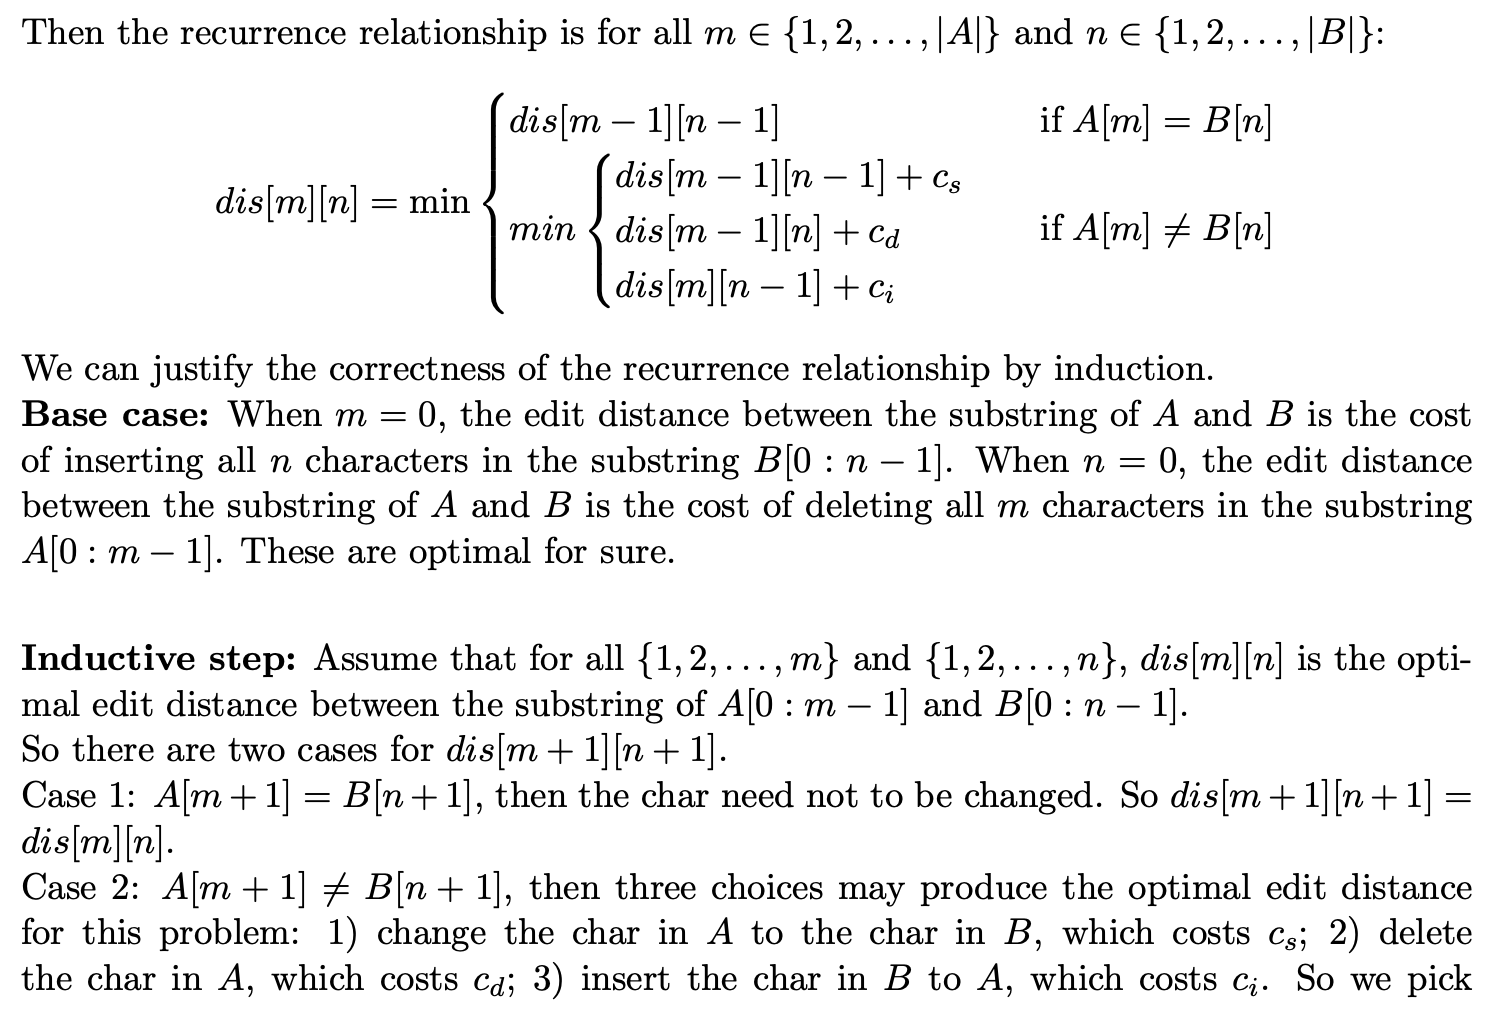
\includegraphics[scale=0.5]{1.png}\\
    \end{center}
    I think I did fair enough in hw 2, giving mostly correct answers, especially in the greedy algorithm part. I think I could have done better in the dynamic programming part. In problem 4, I took the fact that in the case when $A[i] = B[i]$, $ED(i-1, j-1)$ is the most efficient way but did not rigorously prove it. Next time I should think more carefully. 
    \end{solution}

    \question \textbf{Decision Problems and Languages.} \textcolor{blue}{(L8)}
    
Recall that the goal of a \emph{decision problem} is to determine whether a given input ``object'' has a certain ``property'', e.g., determine whether a given integer is prime, or whether a given string is a palindrome.
  In class, we said that any decision problem is equivalent to a \emph{membership problem} for a corresponding \emph{language}.
  That is, determining whether a given object has the property is equivalent to determining whether its encoding (as a string) is a member of the language.

  For each of the following decision problems, (i)~define a reasonable (finite) alphabet~$\Sigma$, (ii)~give the encoding (over the alphabet) of a representative input object, (iii)~analyze the length of the encoding in terms of the value of the input, and (iv) define a language~$L$ for the corresponding decision problem.
  Use the notation~$\inner{X}$ for the encoding of object~$X$ as a string over the alphabet.
  As examples, we have provided solutions to the first two parts. 
    
  \begin{parts}
    \part \textbf{Example:} ``Does a given non-negative integer $k$ have 3 as its last digit, when written in base 10?''
    
    \begin{solution}
      \begin{enumerate}[(i)]
      \item A reasonable alphabet consists of the decimal digits, $\Sigma = \set{\texttt{0}, \ldots, \texttt{9}}$.
      Alternatively, we could use the binary digits $\bit$, or hexadecimal digits (0 through 9 and A through F), or the digits from any other base (including unary), or some entirely different-looking alphabet like $\set{\star, \otimes, \bot}$ (though the latter would not be very human-friendly).
      No matter the choice of (nonempty, finite) alphabet, there is a way to unambiguously encode (represent) non-negative integers as strings of characters from that alphabet.

      Note that it would \emph{not} be valid to include all of the non-negative integers in the alphabet, because an alphabet must be a \emph{finite} set, and there are infinitely many non-negative integers.

      \item Example encoding: For an integer $k$, write it in base 10 in the usual way, as a string of digits.
        For example, if $k$ is the integer forty-seven, then $\langle k \rangle = \texttt{47}$.
        We stress that this is a \emph{string} of the characters \texttt{4} and \texttt{7}, which \emph{represents} the number forty-seven.

      \item The length of this encoding would be the number of digits in the value, which is $\Theta(\log k)$.

      \item A corresponding language would be $L_{EndsWith3} = \set{\langle k \rangle : k \bmod 10 = 3}$.
        It would also be acceptable to copy the phrasing of the decision problem, i.e., $L_{EndsWith3} = \set{\langle k \rangle : k \text{ written in base 10 has 3 as the last digit}}$
      \end{enumerate}

      Alternatively, we could also encode integers in binary, using the alphabet $\Sigma=\set{0,1}$.
      For example, if $k=5$, then $\langle k \rangle = \texttt{101}$.
      The length of this encoding is still $\Theta (\log k)$.
      The above two definitions of the language hold without modification, because they both describe membership only in terms of the \emph{value} of~$k$, not its encoding.
    \end{solution}
    
    \part \textbf{Example:} ``Is a given array of non-negative integers sorted?''
    
    \begin{solution}
      \begin{enumerate}[(i)]
      \item A reasonable alphabet $\Sigma$ is the set of ASCII characters, or more selectively, the decimal digits along with some separator characters: $\Sigma = \set{\texttt{0}, \ldots, \texttt{9}, \texttt{[}, \texttt{,}, \texttt{]}}$.
        (Notice that a comma is one of these characters.)

        Note that we can't just use the decimal digits alone if we also want some special symbols to indicate the start/end of the array and to separate the elements.
          
      \item Example encoding: For an array $A$, encode its elements as in the previous part, and list those encodings with appropriate separators.
        For example, the array $A$ with entries one, two, three, and four would have $\langle A \rangle = \texttt{[1,2,3,4]}$.
      \item The length of this encoding is $\Theta(n + e)$, where~$n$ is the number of elements in the array, and $e$ is the total length of the encodings of the elements.
      \item The corresponding language is \[ L_\text{sorted} = \set{\langle A \rangle : A \text{ is a sorted array of non-negative integers.}}
          .
        \]
      \end{enumerate}
    \end{solution}
    
    \part [4] ``Given two strings compost of English alphabets, do they have a common subsequence of length $k$?''

    \begin{solution}
    \begin{enumerate}[(i)]
      \item A reasonable alphabet $\Sigma$ is the set of 26 English letters both in their upper and lower case forms, together with a quotation mark for : $\Sigma = \set{\texttt{a}, \ldots, \texttt{z}, \texttt{A}, \ldots, \texttt{Z}, \texttt{[}, \texttt{,}, \texttt{]}}$.  
      \item Example encoding: For an array $A$, encode its elements as in the previous part, and list those encodings with appropriate separators.
        For example, the array $A$ with entries one, two, three, and four would have $\langle A \rangle = \texttt{[1,2,3,4]}$.
      \item The length of this encoding is $\Theta(n + e)$, where~$n$ is the number of elements in the array, and $e$ is the total length of the encodings of the elements.
      \item The corresponding language is \[ L_\text{sorted} = \set{\langle A \rangle : A \text{ is a sorted array of non-negative integers.}}
          .
        \]
      \end{enumerate}
    \end{solution}
    
    \part [4] ``Does a given undirected graph $G$ has a Hamiltonian cycle?" \textit{Hint: Consider adjacency matrix.} 

     \begin{solution}

    \end{solution}

    \end{parts}

    \question \textbf{DFAs.} \textcolor{blue}{(L8)}

    For this problem, check out \href{https://madebyevan.com/fsm/}{this tool} to generate \texttt{tikzpicture} script for your DFA. 

    \begin{parts}
        \part [4] Consider the following DFA: 
        \begin{center}
        \begin{tikzpicture}[shorten >=1pt,node distance=2cm,on grid,auto]
           \node[state,initial] (q_0)   {$q_0$}; 
           \node[state] (q_1) [right=of q_0] {$q_1$};
           \node[state,accepting] (q_2) [right=of q_1] {$q_2$};
           \path[->]
            (q_0) edge [loop above] node {$b$} ()
                  edge node {$a$} (q_1)
            (q_1) edge [loop above] node {$b$} ()
                  edge node {$a$} (q_2)
            (q_2) edge [loop right] node {$a, b$} ();
        \end{tikzpicture}
        \end{center}
        Determine the (i) alphabet, (ii) state-transition function and (iii) language decided by the DFA. You may describe the language in English or regular expression, whichever you prefer.
        \begin{solution}
        
        \end{solution}

        \part [5] Give a DFA that decides language $L$ over the alphabet $\set{a,b}$ corresponding to the regular expression $a^*ba^*(ba^*ba^*)^*$. You may represent the DFA as a state-transition function or as a diagram, whichever you prefer. 

        \begin{solution}
            
        \end{solution}

        \part [6] Give a DFA that decides the following language over the alphabet $\Sigma = \set{a,b}$
        \[
            L = \set{s \in \Sigma^*: s \text{ contains at least two $a$'s \textbf{and} odd number of $b$'s.}}.
        \]
        You may represent the DFA as a state-transition function or as a diagram, whichever you prefer.

        \begin{solution}
        
        \end{solution}
        
    \end{parts}

    \question \textbf{Turing Machines Potpourri.} \textcolor{blue}{(L9, L11)}

    Determine whether the following statements about Turing Machines are always/ sometimes/ never true. While justification is \textbf{not required} to received for full credit, providing it is highly encouraged.
    
    \begin{parts}

    \part [3] A language that is decidable by a DFA is (always/ sometimes/ never) decidable by a Turing machine. 
    \begin{solution}
    
    \end{solution}
    
    \part [3] A Turing machine will (always/ sometimes/ never) halt before reading in its full input.
    \begin{solution}
    
    \end{solution}
    
    \part [3] If a Turing machine does not halt on a given input, then the number of cells written to on its tape for that input is (always/ sometimes/ never) unbounded.
    \begin{solution}
    
    \end{solution}

    \part [3] If a given Turing machine is guaranteed to only write to a finite number of cells on a tape, then it would (always/ sometimes/ never) halt.
    \begin{solution}
    
    \end{solution}

    \part [3] A Turing machine can (always/ sometimes/ never) decide its own halting problem.
    \begin{solution}
    
    \end{solution}
    
    \end{parts}


  \question \textbf{A Powerful Diagonalization.} \textcolor{blue}{(L10)}

  \begin{parts}

    \part[7] The \emph{power set} of a set $A$, denoted $\mathcal{P}(A)$, is defined as the \emph{set of all subsets} of~$A$.
    For example, $\mathcal{P}(\bit)=\set{\emptyset,\set{0},\set{1},\bit}$.
    
    Use diagonalization to prove that for any \emph{countably infinite} set~$A$, the power set $\mathcal{P}(A)$ is \emph{uncountably} infinite.
    
    \hint{View each subset as an infinite binary sequence representing whether each element of~$A$ is included in the subset or not.}
    
    \begin{solution}
 
    \end{solution}
    
    \part[7] Prove that any infinite language $L \subseteq \Sigma^*$ has an undecidable subset $L' \subseteq L$.
    
    \hint{Part (a) will be useful.}
    
    \begin{solution}

    \end{solution}
  \end{parts}

    \question \textbf{Decidability and Set Operations.} \textcolor{blue}{(L11)}
     
     Consider four languages where $L_{D1}$ and $L_{D2}$ are decidable, and $L_{U1}$ and $L_{U2}$ are undecidable. Determine whether the following languages are always/ sometimes/ never decidable. The case of $L_{D1} \cap L_{D2}$ is provided as an example. While justification is \textbf{not required} to received for full credit, providing it is highly encouraged.

     \begin{parts}
         \part \textbf{Example:} $L_A = L_{D1} \cap L_{D2}$

         \begin{solution}
             \textbf{Always.} Let $M_1$ be a TM that decides $L_{D1}$, and $M_2$ be a TM that decides $L_{D2}$. We use these to construct the following Turing Machine that decides $L_{D1}\cap L_{D2}$:
            \begin{center}
                \begin{minipage}{0.8\linewidth}
                    \begin{algorithm}[H]
                        \algorithmiconinput{$M'$}{($x$)}
                        \begin{algorithmic}[1]
                            \State Run $M_1$ on $x$ and run $M_2$ on $x$
                            \State \textbf{If} both $M_1$ and $M_2$ accepted $x$ \textbf{then} accept
                            \State \textbf{Else} reject
                        \end{algorithmic}
                    \end{algorithm}
                \end{minipage}
            \end{center}
            \textbf{Analysis:}
            \begin{itemize}
                \item $x \in (L_{D1} \cap L_{D2}) \implies x \in L_{D1} \land x \in L_{D2} \implies M_1 \text{ accepts } \land M_2 \text{ accepts } \implies M \text{ accepts}$
                \item $x \notin (L_{D1} \cap L_{D2}) \implies x \notin L_{D1} \lor x \notin L_{D2} \implies M_1 \text{ rejects } \lor M_2 \text{ rejects } \implies M \text{ rejects}$
            \end{itemize}
            Since $M_1$ and $M_2$ are deciders, they necessarily halt on all inputs. Thus, $M'$ must also halt on all inputs. In addition, since $M'$ accepts all $x \in (L_{D1} \cap L_{D2})$ and rejects all $x \notin (L_{D1} \cap L_{D2})$, it follows that $M'$ decides $L_{D1} \cap L_{D2}$. As we have constructed a decider for $(L_{D1} \cap L_{D2})$, we can conclude that $(L_{D1} \cap L_{D2})$ is necessarily decidable.
         \end{solution}
         \part [4] $L_B = L_{D1} \cup L_{D2}$
         \begin{solution}

         \end{solution}
         
         \part [4] $L_C = L_{D1} \cap L_{U1}$
         \begin{solution}

         \end{solution}
         
         \part [4] $L_D = L_{D1} \cup L_{U1}$
         \begin{solution}

         \end{solution}
         
         \part [4] $L_E = L_{U1} \cap L_{U2}$
         \begin{solution}

         \end{solution}
         
         \part [4] $L_F = L_{U1} \cup L_{U2}$
         \begin{solution}

         \end{solution}
     \end{parts}

 \question \textbf{Can You Decide?}

    For each of the following language, determine with proof whether the language is decidable or not. If decidable, describe and analyze a Turing machine that decides it. If undecidable, prove that reduce it from some language $L$ of your choice that we have previously proved is undecidable.

    \begin{parts}
        \part [6] $\LOddF = \set{x \in \{0, 1, 2, 3, 4\}^*: x \text{ represents an odd number in base 5} }$. \textcolor{blue}{(L11)}
        
        \begin{solution}

        
        \end{solution}

        \part [6] $L_{\text{AND-LOOP}} = \set{(\langle M\rangle,x,y) : M \text{ is a TM that loops on input $x$ and loops on input $y$}}$ \textcolor{blue}{(L11)}
    
        \begin{solution}

        \end{solution}

    \part[6] Consider a language $\LIMFinite$ that contains a finite number of strings. Is $\LIMFinite$ (always/ sometimes/ never) decidable? Justify your answer. \textcolor{blue}{(L11)}

    \begin{solution}

    \end{solution}
    
    \bonuspart \textit{This part is optional and ungraded for this homework, but it's} \textbf{within the scope of the midterm}. \textit{Therefore, we highly encourage you to attempt the problem.} 
    
    Define the language \[\LFinite = \set{ \inner{M} : M \text{ is a Turing machine and $L(M)$ is finite} }. \] Determine whether $\LFinite$ is decidable or undecidable. If decidable, describe and analyze a Turing machine that decides it. If undecidable, prove that $L \leq_T \LFinite$ for some language $L$ of your choice that we have previously proved is undecidable. \textcolor{blue}{(L12)}
    
    \begin{solution}

    \end{solution}
    \end{parts}
    
\end{questions}

\end{document}